\chapter{Teakwood System }

\section{Overview}
Structurally, like most websites, Teakwood system has a three layer layout: frontend, backend, and database. Becuase Teakwood will use computing servers to run jobs, so The eco Teakwood system actually has four layers, the up mentioned three plus the computing layer. the below figure shows how it looks like.\\

\begin{figure}[htb]
\centering
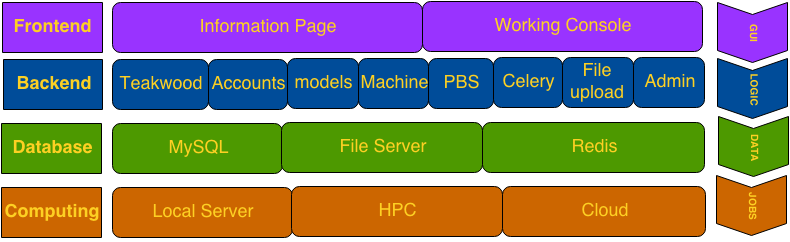
\includegraphics[scale=0.5]{./system_structure} 
% e.g. insert ./image for image.png in the working directory, adjust scale as necessary
\caption{Teakwood System Overview}
\label{fig:label} % insert suitable label, this is used to refer to a fig from within the text as shown above
\end{figure}

On the above figure, we can see four straight layers bottom up. In each layer, the left part is the layer name, the middle part is the layer content, and the right part is what its actally is. We will go through details one by one.

\section{Frontend}
The frontend is the visible GUI that user interact with. Basically all what we can see from the Teakwood website can be called "frontend".  For neat purpose, I separated the frontend into two parts: the information page and the working console. see below:

\begin{figure}[htb]
\centering
%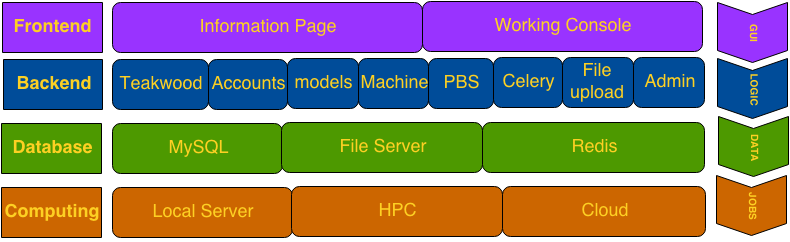
\includegraphics[scale=0.5]{./system_structure} 
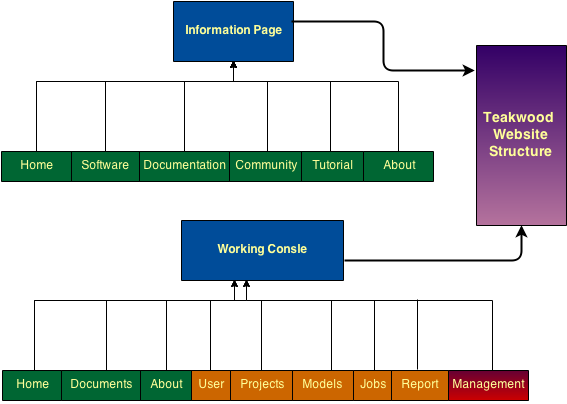
\includegraphics[scale=0.6]{./website_structure} % e.g. insert ./image for image.png in the working directory, adjust scale as necessary
\caption{Website Strucutre}
\label{fig:label} % insert suitable label, this is used to refer to a fig from within the text as shown above
\end{figure}

The infomation page gives you all things about Teakwood.\\

$\bullet$What is teakwood?\\
$\bullet$What can Teakwood do?\\
$\bullet$How to install teakwood?\\
$\bullet$How to use Teakwood?\\
$\bullet$The user manual.\\
$\bullet$Video tutorial.\\
$\bullet$Teakwood forum.\\

Note the color differences in the bottom layer.\\

$\bullet$The Green: all visitor can see and manipulate.\\
$\bullet$The orange: only logged user can see and manipulate.\\
$\bullet$The red: only superuser can see and manipulate.\\

This logic is achieved by desiang a if-else template structure, and the authentication function is provided by Django itself.


\section{Backend}
The backend is the logical design of handling data. Teakwood system follows the loose-coupling design manner, so she separated the logic in to different parts, any changes in one part will not mess other parts. (We will have a backend chapter to reveal the logic mystery.)
In Teakwood system, there are mainly eight big logic designs.\\

$\bullet$ \textbf{Teakwood}: control the frontend presentation.\\
$\bullet$ \textbf{Accounts}: control the user identification.\\
$\bullet$ \textbf{Models}: invoke and control the computing models.\\
$\bullet$ \textbf{machine}:invoke and control the computing resources\\
$\bullet$ \textbf{PBS}:Guide the PBS script generation.\\
$\bullet$ \textbf{File upload}:achieve the input files gathering function\\
$\bullet$ \textbf{Admin}:overall control of user and data.\\
$\bullet$ \textbf{Celery}:asynchronous handling.\\

\section{Data handling}
Teakwood system handles three types of data: the website data, the computing data and the message queue data. For each type of data we provide a different storage. see this table:
\begin{table}[h]
\begin{tabular}{lllll}
\cline{1-3}
\multicolumn{1}{|c|}{\textbf{Website data}} & \multicolumn{1}{c|}{\textbf{Computing data}} & \multicolumn{1}{c|}{\textbf{Message queue data}} &  &  \\ \cline{1-3}
\multicolumn{1}{|c|}{\textbf{Database}} & \multicolumn{1}{c|}{\textbf{File server}} & \multicolumn{1}{c|}{\textbf{redis server}} &  &  \\ \cline{1-3}
\multicolumn{1}{|c|}{\textbf{data in Teakwood}} & \multicolumn{1}{c|}{\textbf{nputs and outputs}} & \multicolumn{1}{c|}{\textbf{Asynchronous handling}} &  &  \\ \cline{1-3}
                                &                                &                                &  & 
\end{tabular}
\end{table}

Teakwood system uses MySQL database for store it website data.
Teakwood periodically rsync server data to Teakwood file server for backup purpose.
Messge queue key-values are ephemeral data, so we simply use a redis server to keep it.
\section{Remote Configuration}
Before the first time we can use remote computing resources, we have set up a connection and ready everthing. the main things we should done are:\\

$\bullet$ Establish an passwordless ssh login.\\
$\bullet$ Compile the tools/packages we will use in remote machine.\\
$\bullet$ Ready all the import path for Teakwood to use.


%\subsection{<Sub-section title>}

%\subsection{<Sub-section title>}
%some text\cite{citation-2-name-here}, some more text

%Refer figure \ref{fig:label}.


